% Pebre
\newpage
%\thispagestyle{empty}
\begin{recipe}[source={Receta del Papá},
preparationtime={\unit[10-15]{Minutos}}
]{Pebre}
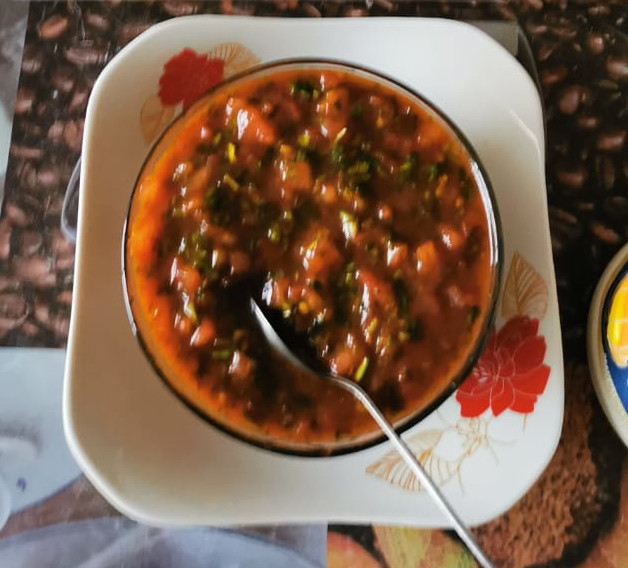
\includegraphics[width=0.25\textwidth]{pebre}
\introduction{
Este pebre es tradicional en los asados familiares, es ligeramente picante, muy rico y combina muy bien con el choripán, carne y hasta puede ser simplemente un acompañamiento para el pan.
}
\ingredients{
    2 & Tomates \\
    3 & Dientes de Ajo \\
    1 & Manojo de perejil \\
    1 & Manojo de cilantro \\
    1 & Bolsita de pasta de ají \\
	& Aceite de oliva a gusto \\
	1 & Cucharadita de sal. (A gusto)
}
\preparation{
    \begin{enumerate}
        \item Pelar los tomates y picar en cubitos finos.
        \item Pelar y picar finamente los dientes de ajos.
        \item Picar finamente el perejil y el cilantro.
        \item En un recipiente, verter los tomates picados, el cilantro, el perejil, el ajo, la pasta de ají, agregar un poco de aceite de oliva y la sal.
        \item Revolver hasta que todo esté mezclado.
        \item Refrigerar por al menos 15 minutos y ya está listo para servir.
    \end{enumerate}
}
\end{recipe}